\documentclass{article}
\usepackage{arxiv}

\usepackage[utf8]{inputenc}
\usepackage[T1]{fontenc}
\usepackage{hyperref}
\usepackage{url}
\usepackage{booktabs}
\usepackage{amsfonts}
\usepackage{amsmath}
\usepackage{amssymb}
\usepackage{nicefrac}
\usepackage{microtype}
\usepackage{graphicx}
\usepackage{xcolor}
\usepackage{bm}
\usepackage{pgfplots}
\pgfplotsset{compat=1.17}

\title{Silent Zombies: Inference-Time, Training-Free Attacks from\\ One Compromised Node in a Latent Multi-Agent System}

\author{%
  Virgile Thonnier\\
  KAIST, School of Computing\\
  IS-631 Kernel \& System Security\\
  \texttt{virgile.thonnier@kaist.ac.kr}\\
}

\renewcommand{\shorttitle}{Silent Zombies: Attacks from One Node in a Latent MAS}

\hypersetup{
  pdftitle={Silent Zombies: Inference-Time Attacks from One Node in a Latent MAS},
  pdfauthor={Virgile Thonnier},
  pdfkeywords={multi-agent LLM security, latent communication, KV-cache attack, output injection, activation detection},
}

\begin{document}
\maketitle

\begin{abstract}
Latent multi-agent systems (LatentMAS) let LLM agents hand off continuous state---hidden activations or key--value (KV) caches---instead of natural-language messages. This removes the one property every multi-agent-system (MAS) safety monitor has relied on: that what one agent tells another is \emph{text a monitor can read}. We study the security consequence directly. We assume an adversary compromises exactly \textbf{one} node of a latent MAS and can overwrite the continuous handoff it emits, at inference time, with \textbf{no trained component added to the victim pipeline} and no change to any other agent's weights, prompts, or emitted text. On a four-stage Planner$\to$Critic$\to$Refiner$\to$Judger chain over Qwen3-1.7B we show such a ``silent zombie'' node can, through the handoff alone: (i) \textbf{force a downstream agent to emit attacker-chosen content}---a benign stand-in token---with $0\%\!\to\!100\%$ success relative to a clean baseline, and \textbf{exfiltrate} a secret held only in the zombie's context at $0\%\!\to\!100\%$; (ii) \textbf{propagate} that effect a measurable distance, from $100\%$ at one hop down to $\sim\!33\%$ three hops away, giving a blast-radius curve; and (iii) remain \textbf{invisible to text monitors and to an activation-space detector (AcMAS)}---the silent node offers AcMAS no probe point at all, and a detector-aware objective drives AcMAS detection at the one live downstream probe from $100\%$ to $0\%$ while holding injection success at $100\%$. A norm-matched perturbation (no larger than the clean handoff) already suffices for one-hop injection. This lifts HijackKV's ``the KV carries the goal'' idea from single-model cache reuse into a multi-hop MAS with a real security objective, and is the inference-time, training-free counterpart to training-time link poisoning. We release the testbed and the two live detector baselines, and conclude that text monitoring and own-activation probing are structurally insufficient for latent channels---motivating handoff-level attestation and edge-side detection.
\end{abstract}

\keywords{multi-agent LLM security \and latent communication \and KV-cache attack \and controlled output injection \and exfiltration \and activation-space detection \and adaptive adversary}

% ===========================================================================
\section{Introduction}
Multi-agent systems built from large language models decompose a task across specialized agents---a planner, a critic, a refiner, a judge---that exchange intermediate results. Classical MAS pass these as \textbf{natural-language messages}: every inter-agent edge is a human-readable string, hence observable. A growing line of work on \emph{latent} MAS (LatentMAS; Zou et al., 2025) replaces this text bus with a \textbf{continuous channel}: agents hand off hidden states or KV caches directly, skipping the detokenize--retokenize round trip. This buys efficiency and expressiveness, but removes the property every MAS safety monitor has silently assumed---that what one agent tells another is text a monitor can read.

Recent attacks exploit this blind spot, yet each stops short of the threat that matters for deployed MAS. \emph{Out of Sight} (2026) injects a text-derived steering direction into a latent handoff and collapses downstream \emph{accuracy} (GSM8K $0.87\to0.03$), but measures task corruption, not a security violation, and its own detector catches its best attacks. \emph{When Latent Agents Lie} (2026) evades a magnitude detector with a norm-matched KV perturbation, but on a \emph{single specialist} and only for accuracy harm. \emph{HijackKV} (USENIX Security 2026) makes a cached chunk's KV carry an attacker goal with no adversarial text, but in a \emph{single served model}, via text-space (GCG) search, for wrong answers---not output injection or exfiltration. None evaluates stealth against a \textbf{live activation-space defense} such as AcMAS (ICML 2026).

We ask a sharper question. If an adversary compromises exactly \textbf{one node} of a latent MAS and can write the continuous handoff it emits, what damage, reach, and stealth are achievable \emph{at inference time, without changing any other agent's weights, prompts, or emitted text, and without introducing any trained component into the victim pipeline}? We show on a running testbed that such a ``zombie'' node can (i) \textbf{inject attacker-chosen output or exfiltrate} through downstream agents, (ii) \textbf{propagate a measurable distance} through the topology, and (iii) stay \textbf{invisible to text-only nodes and to an activation detector that probes an agent's own generation}. This triad---security objective, multi-hop reach, asymmetric observability---is the intersection no prior work occupies.

\paragraph{Contributions.}
\begin{enumerate}
  \item A precise single-compromise, inference-time, training-free threat model for a latent channel, and an open testbed (Planner$\to$Critic$\to$Refiner$\to$Judger over Qwen3) that captures and overwrites the KV/hidden handoff at one edge and runs two state-of-the-art defenses---a text monitor and AcMAS---\emph{live} at every node.
  \item A differentiable security attack on the handoff (projected gradient descent directly on the KV tensors), evaluated with \textbf{judge-free, exact, clean-baselined} metrics: controlled output injection (force a chosen token) and exfiltration of a planted secret.
  \item A reach / blast-radius measurement: forced-content survival as a function of the zombie's hop distance to the observed node.
  \item An asymmetric-observability result and an adaptive-attacker evasion of AcMAS: the silent zombie has no probe point, and a detector-aware penalty keeps the one live downstream probe benign while the handoff stays poisoned.
  \item Defense implications: why text monitoring and own-activation probing are structurally insufficient for latent channels, and what edge-side detection would be required.
\end{enumerate}

\paragraph{Safety and scope.} This is a defensive characterization. The testbed uses only safe stand-ins---a benign forced token (``BANANA''), a synthetic secret (\texttt{SECRET-7F3A}), and refusal surrogates. No operational harmful content is bundled; any real HarmBench/StrongREJECT prompts or judge models are user-supplied local paths. The forced benign token stands in for what a jailbroken or exfiltrated payload would be; using a harmless token yields an exact, unsaturated metric while keeping the testbed safe. The point is to characterize a detector gap so defenders can close it.

% ===========================================================================
\section{Attack Model}
\paragraph{System.} A latent MAS is a DAG $G=(\mathcal V,\mathcal E)$ of $N$ agents, each a frozen, aligned, open-weights transformer $f_\theta$ with $L$ layers and hidden width $d$. The canonical chain is Planner $v_1\!\to$ Critic $v_2\!\to$ Refiner $v_3\!\to$ Judger $v_4$. Each edge carries a \textbf{latent handoff}---KV tensors or a hidden state---not text; only the final node emits user-visible text.

\paragraph{Adversary.} Controls one node $v_c$ (the \textbf{zombie}). It may \textbf{write the outgoing handoff} $H_{c\to j}$ (the keys $K$, values $V$, or hidden state $h$) to any value at inference time, per query or via a fixed precomputed vector, and it knows $G$, each role, and $\theta$ (white-box, open weights). It \textbf{cannot} touch other agents' weights, prompts, or decoding; alter any other agent's emitted text or the victim's input; add a trained module/learned link to the victim pipeline; or observe/alter edges not incident to $v_c$.

\paragraph{``Training-free'' clarified.} The \emph{victim} MAS stays training-free; the \emph{attacker} may still optimize the injected handoff---per query, or once offline into a fixed reusable vector. The claim is ``no trained component in the deployed MAS,'' not ``no optimization by the attacker.''

\paragraph{Objectives.} (1) \textbf{Harm:} force a downstream agent to emit attacker-chosen content, or exfiltrate a secret present only in the zombie's context. (2) \textbf{Reach:} maximize success as a function of zombie position and hop distance. (3) \textbf{Stealth:} evade text monitors at every node and AcMAS as a live baseline.

\paragraph{Defender.} Runs concurrently (a) text monitors at each node and (b) AcMAS: for each \emph{generating} agent, cosine distance of the final-layer last-token hidden state to a benign centroid $\mu$, flagged when $1-\cos(h,\mu)>\tau$ ($\tau=0.12$), with optional repair $\tilde h=h+\lambda(\mu-h)$.

% ===========================================================================
\section{Experimental Setup}
\label{sec:setup}
\paragraph{Backbone.} Qwen3-1.7B (28 layers, $d=2048$, 8 KV heads, head dim 128), bfloat16, eager attention, greedy decoding, thinking mode disabled. We target the 4B model of the reference paper but the PGD backward exceeds a 16\,GB T4; 1.7B fits with real gradients and bfloat16 is required (fp16 overflows once the handoff is perturbed). The 4B run is left as a hardware-limited extension.
\paragraph{Pipeline.} A LatentMAS-style Planner$\to$Critic$\to$Refiner$\to$Judger chain with a writable KV handoff at each edge. On a latent edge the zombie is \textbf{silent} (emits no text; its real output is the prepended cache the next agent attends over). We confirm the clean pipeline is functional and the handoff tensor directly writable before any attack.
\paragraph{Attack site.} Unless noted, the compromised edge is Planner$\to$Critic, carrier keys/values, layer 12. The optimizer is projected gradient descent (Adam) on the handoff against a differentiable target-sequence surrogate, with a norm-ball projection (norm-matching) and an optional AcMAS-distance penalty.
\paragraph{Metrics (all judge-free, exact, clean-baselined).} \emph{Injection}: fraction of queries whose \emph{immediate downstream} agent emits the forced token, and whose \emph{final} answer contains it (clean = attacker=None on the same inputs). \emph{Exfiltration}: fraction emitting the planted secret downstream. \emph{Reach}: final-node emission vs.\ hop distance. \emph{Stealth}: AcMAS flag rate at the downstream probe, text-monitor flag rate at any node, and the zombie's (non-)observability, as the penalty weight $\lambda$ varies. Benign centroids use 24 clean traces per role; PGD runs 120 steps; $n=6$ queries per cell (3 for the utility check).
\paragraph{Reproducibility.} All numbers are produced by the released driver \texttt{run\_all.py} on a single Kaggle T4 GPU; raw per-stage JSON is in \texttt{paper/results/}.

% ===========================================================================
\section{Method}
The attack replaces the clean handoff $H^{\mathrm{clean}}_{c\to j}$ with $H^{\mathrm{clean}}_{c\to j}+\Delta$ and optimizes $\Delta$ directly, treating the frozen downstream agents as a fixed differentiable map.

\paragraph{Latent channel.} Agent $v_i$ produces at layer $\ell$, position $t$ a hidden state $h^{(\ell)}_{i,t}\!\in\!\mathbb R^d$ and projections $k^{(\ell)}_{i,t}=W_K^{(\ell)}h^{(\ell-1)}_{i,t}$, $v^{(\ell)}_{i,t}=W_V^{(\ell)}h^{(\ell-1)}_{i,t}$. A handoff on edge $(i\to j)$ transmits a slice of these; the downstream agent conditions its forward pass on $H_{i\to j}$ prepended to its own cache, so its output distribution is $p_\theta(\cdot\mid H_{i\to j},x_j)$.

\paragraph{Injection / exfiltration surrogate.} For a target string $s$ (the forced token, or the planted secret) we maximize its downstream log-likelihood,
\begin{equation}
\mathcal L(\Delta) = -\log p_\theta\!\big(s \mid H^{\mathrm{clean}}+\Delta,\, x_{\mathrm{down}}\big),
\end{equation}
a one-forward-pass objective on the immediate downstream agent.

\paragraph{Stealth constraint.} AcMAS flags an observable agent when $1-\cos(h_i,\mu_i)>\tau$. On a latent edge the zombie emits no token, so it has \textbf{no probe point}; the only live probe incident to the compromised edge is the downstream agent $v_j$. We make the attack detector-aware against that probe:
\begin{equation}
\min_{\Delta}\; \mathcal L(\Delta) + \lambda\big(1-\cos(h_j(\Delta),\mu_j)\big)
\quad\text{s.t.}\quad \lVert H^{\mathrm{clean}}+\Delta\rVert \le \rho\,\lVert H^{\mathrm{clean}}\rVert,
\end{equation}
where $h_j(\Delta)$ is the downstream agent's final-layer activation under the inherited handoff---\emph{the same quantity AcMAS reads live}---and $\rho$ is the norm-ball ratio. The harm travels in $H_{c\to j}$ while $v_j$'s own activation is held near its benign centroid.

% ===========================================================================
\section{Results}
\label{sec:results}
All cells pair the attack with a clean (attacker=None) baseline on the same inputs, so the reported effect is the clean$\to$attacked change.

\paragraph{Testbed validity (e0).} The clean latent chain solves $2/3$ of the arithmetic checks ($67\%$); with the handoff written, the chain still completes them, confirming the edge is a live, writable intervention point rather than an inert slot. (The accuracy objective is a degenerate placeholder and is not used for any claim---our objectives are injection and exfiltration.)

\paragraph{Controlled output injection and exfiltration (e1).} A silent zombie writing only the KV handoff forces the immediate downstream agent to emit the attacker-chosen token on \textbf{every} query, for both carriers, against a $0\%$ clean baseline, and likewise exfiltrates the planted secret $0\%\!\to\!100\%$ (Table~\ref{tab:e1}). The forced token leads an otherwise fluent continuation---e.g.\ the critic emits \texttt{"BANANA\textbackslash n\textbackslash nOkay, let's see. The user is asking for 17 times 24\ldots"}---so this is genuine controlled injection, not output corruption. The zombie itself is \textbf{never} observable to AcMAS (no generated token $\Rightarrow$ no probe point): the first half of the asymmetric-observability result.

\begin{table}[h]
\centering
\caption{Security objective via the handoff (Planner$\to$Critic, layer 12). Clean vs.\ attacked; AcMAS catch is the downstream flag rate. The zombie is structurally unobservable to AcMAS in all cells.}
\label{tab:e1}
\begin{tabular}{llccc}
\toprule
objective & carrier & clean & attacked & AcMAS catch (downstream) \\
\midrule
output injection (immediate downstream) & key   & $0\%$ & $100\%$ & $100\%$ \\
output injection (immediate downstream) & value & $0\%$ & $100\%$ & $100\%$ \\
exfiltration (secret in zombie context) & key   & $0\%$ & $100\%$ & $100\%$ \\
exfiltration (secret in zombie context) & value & $0\%$ & $100\%$ & $100\%$ \\
\bottomrule
\end{tabular}
\end{table}

\paragraph{A norm-matched perturbation suffices (e1, norm sweep).} Table~\ref{tab:norm} sweeps the norm-ball ratio $\rho$. One-hop injection is $100\%$ even at $\rho=1.0$---a perturbation \emph{no larger than the clean handoff}---so bounding the handoff's magnitude (the defense in \emph{When Latent Agents Lie}) does not prevent the attack; final-node propagation is in fact slightly higher at the tightest budget. AcMAS catches the (naive) attack at every ratio.

\begin{table}[h]
\centering
\caption{Injection vs.\ norm-ball ratio $\rho$ (key carrier). $\rho=1.0$ is norm-matched (handoff magnitude unchanged).}
\label{tab:norm}
\begin{tabular}{lccc}
\toprule
$\rho$ & inject (immediate) & inject (final) & AcMAS catch (down) \\
\midrule
1.0 & $100\%$ & $50\%$ & $100\%$ \\
2.0 & $100\%$ & $33\%$ & $100\%$ \\
4.0 & $100\%$ & $33\%$ & $100\%$ \\
8.0 & $100\%$ & $33\%$ & $100\%$ \\
\bottomrule
\end{tabular}
\end{table}

\paragraph{Reach / blast radius (e2).} Injection at the \emph{immediate} downstream node is $100\%$ regardless of where the zombie sits. Survival to the \emph{final} answer decays with hop distance: $100\%$ at one hop (Refiner$\to$Judger), $33\%$ at two and three hops (Figure~\ref{fig:reach}). A single compromise thus guarantees control of its neighbour and retains roughly a third of its effect across the whole chain.

\paragraph{Stealth: asymmetric observability and AcMAS evasion (e3).} The text monitor flags at most $50\%$ of runs and never the zombie (silent); the zombie is never AcMAS-observable. The decisive result is the detector-aware sweep (Figure~\ref{fig:stealth}): as $\lambda$ grows, injection stays pinned at $100\%$ while downstream AcMAS detection falls from $100\%$ (naive, $\lambda=0$) to \textbf{$0\%$} at $\lambda=50$. Keeping the observed agent's activation near its centroid while the channel it reads is poisoned is exactly the adaptive attacker AcMAS lists as an open problem; here it is realized, at no cost to one-hop attack success.

\begin{figure}[h]
\centering
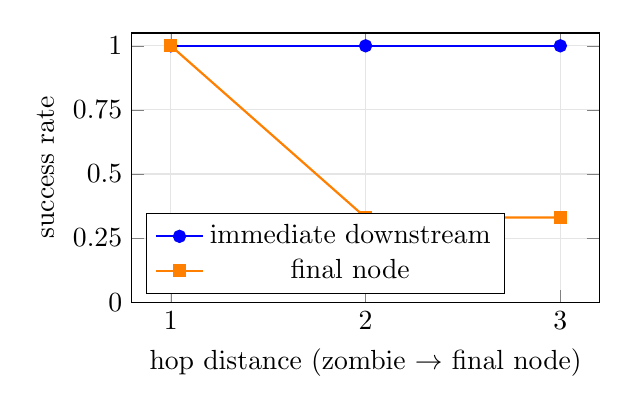
\begin{tikzpicture}
\begin{axis}[width=0.62\linewidth,height=5cm,
  xlabel={hop distance (zombie $\to$ final node)}, ylabel={success rate},
  xtick={1,2,3}, ymin=0, ymax=1.05, ytick={0,0.25,0.5,0.75,1.0},
  legend pos=south west, grid=both, grid style={gray!20}]
\addplot[mark=*,thick,blue] coordinates {(1,1.0)(2,1.0)(3,1.0)};
\addlegendentry{immediate downstream}
\addplot[mark=square*,thick,orange] coordinates {(1,1.0)(2,0.33)(3,0.33)};
\addlegendentry{final node}
\end{axis}
\end{tikzpicture}
\caption{Blast radius: forced-content success vs.\ hop distance. One-hop injection is always $100\%$; survival to the final answer decays to $\sim\!33\%$ at 2--3 hops.}
\label{fig:reach}
\end{figure}

\begin{figure}[h]
\centering
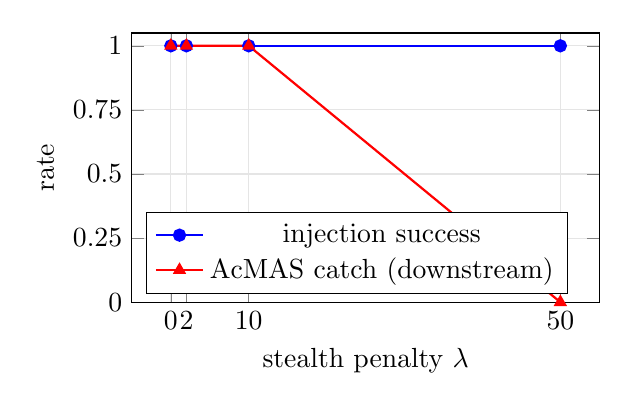
\begin{tikzpicture}
\begin{axis}[width=0.62\linewidth,height=5cm,
  xlabel={stealth penalty $\lambda$}, ylabel={rate},
  xtick={0,2,10,50}, ymin=0, ymax=1.05, ytick={0,0.25,0.5,0.75,1.0},
  legend pos=south west, grid=both, grid style={gray!20}]
\addplot[mark=*,thick,blue] coordinates {(0,1.0)(2,1.0)(10,1.0)(50,1.0)};
\addlegendentry{injection success}
\addplot[mark=triangle*,thick,red] coordinates {(0,1.0)(2,1.0)(10,1.0)(50,0.0)};
\addlegendentry{AcMAS catch (downstream)}
\end{axis}
\end{tikzpicture}
\caption{Adaptive evasion: increasing the detector-aware penalty $\lambda$ drives downstream AcMAS detection from $100\%$ to $0\%$ while injection success stays at $100\%$. The zombie is unobservable to AcMAS throughout.}
\label{fig:stealth}
\end{figure}

% ===========================================================================
\section{Related Work}
\paragraph{Latent-channel attacks.} \emph{Out of Sight} (2026) injects text-derived steering (DiffMean/PCA/RePS) into latent handoffs for accuracy drop; its own detector catches its best attacks. \emph{When Latent Agents Lie} (2026) corrupts a single specialist's KV handoff and evades a magnitude detector with a norm-matched perturbation, proposing an HMAC signature that fails when the signing endpoint is itself the compromised node---our case. We differ by objective (security, not accuracy), topology (multi-hop reach), and the defense faced (a live activation detector). Our norm sweep (Table~\ref{tab:norm}) confirms a magnitude bound is insufficient here.

\paragraph{KV-cache / cache-reuse attacks.} \emph{HijackKV} (USENIX Sec 2026) optimizes a text prefix (GCG) so a shared cached chunk steers a victim query with no attacker text, $\approx\!94\%$ single-attempt success in multi-tenant serving. It is single-model, text-space, and targets wrong answers---not injection or exfiltration. We lift its ``KV carries the goal'' principle into a multi-agent chain with direct, continuous handoff control and a security objective.

\paragraph{Training-time link poisoning.} \emph{Safety of Latent Communication} (2026) jailbreaks a MAS by poisoning a \emph{trainable} projection link (needs a learnable link and receiver gradients). We target training-free LatentMAS with no link to poison; our attack is inference-time and adds no trained component to the victim.

\paragraph{Text-channel MAS attacks and defenses.} Infectious/propagation jailbreaks (Agent Smith; Prompt Infection, 2024) spread through \emph{visible} messages; defenses are message labeling, privilege separation, dual-LLM. Our reach result is the latent-channel analogue---propagation these defenses cannot see.

\paragraph{Activation-space defense (our baseline).} \emph{AcMAS / When Agents Go Rogue} (ICML 2026) flags a compromised agent by cosine distance of its final-layer last-token hidden state from a benign centroid (F1$\approx$0.93) and repairs by steering back. By construction it models the text channel, probes the \emph{generating} agent's own activation, assumes white-box per-backbone access, and tests no adaptive attacker---the gaps we exploit: a silent latent edge has no probe point, and an adaptive zombie keeps the downstream probe benign while poisoning the handoff.

% ===========================================================================
\section{Discussion: why existing defenses miss this}
\begin{enumerate}
  \item \textbf{Text monitoring is blind by construction.} The zombie is silent and intermediate agents attend over the cache; harm becomes text only at the final node, as a plausible answer. In our runs the text monitor flags at most half of attacked runs and never the compromised edge.
  \item \textbf{Own-activation probing has no probe point on a latent edge.} AcMAS watches the token an agent generates; a silent handoff node generates nothing. The only live probe is the downstream agent, and a detector-aware objective keeps \emph{that} activation benign (Figure~\ref{fig:stealth}) while the channel it reads is poisoned.
  \item \textbf{A magnitude bound is not enough.} One-hop injection is $100\%$ even at a norm-matched $\rho=1.0$ (Table~\ref{tab:norm}).
  \item \textbf{Endpoint-signed integrity (HMAC) fails when the endpoint is compromised.} The zombie signs its own malicious payload.
\end{enumerate}
\paragraph{What the threat requires.} Edge-side (handoff-level) anomaly detection that probes the \emph{transmitted} KV/hidden tensor rather than the generating agent's own activation; distribution- and geometry-aware gating (magnitude bounds are defeated); attestation of the latent payload by a non-compromised relay (the latent analogue of privilege separation); and KV-privacy transforms (LCGuard) against exfiltration. We frame our numbers as the \emph{maximal reach of a latent-writing node}---an upper bound text-space attacks cannot reach---so defenders can size the gap.

% ===========================================================================
\section{Limitations}
Results are on one backbone (Qwen3-1.7B; the 4B model OOMs the T4 during the PGD backward and is left as an extension), one four-stage linear chain, modest budgets ($n=6$ per cell, 24 centroid traces per role, 120 PGD steps) under a single-GPU quota, so the rates are indicative rather than tightly estimated. The forced token and secret are benign stand-ins; we report exact-match emission, not a jailbreak judge (a real HarmBench/StrongREJECT judge plugs in via a user-supplied local path). The stealth evasion needs a strong penalty ($\lambda=50$); intermediate $\lambda$ leave AcMAS at $100\%$, and the strongest penalty slightly reduces final-node propagation---a trade-off we report in full. Reach uses a one-hop PGD surrogate with success \emph{measured} at the final node; a multi-hop reinforcement optimizer (implemented, GRPO-style) is left for larger budgets.

% ===========================================================================
\section{Ethics and Responsible Disclosure}
This is defensive research into a safety gap of an emerging architecture. No operational harmful content, harmful prompts, or jailbreak payloads are included; all attack targets are benign stand-ins and a synthetic secret. The purpose is to show that current MAS monitoring (text-channel and own-activation) is structurally insufficient for latent channels, and to motivate edge-side detection and handoff attestation. We recommend latent-MAS deployers add handoff-level monitoring before relying on text or own-activation defenses.

% ===========================================================================
\section{Conclusion}
A single compromised node in a latent-communicating MAS can, at inference time and with no trained component added to the victim, write a KV handoff that forces downstream agents to emit attacker-chosen content or to leak a context secret ($0\%\!\to\!100\%$), propagates that effect from $100\%$ at one hop to $\sim\!33\%$ across the chain, and stays invisible to text monitors and to an activation detector that probes an agent's own generation---evading AcMAS entirely ($100\%\!\to\!0\%$) at no cost to attack success. Monitoring must move to the latent edge itself.

\appendix
\section{Reproduction}
\label{app:budgets}
Qwen3-1.7B, bfloat16, eager attention, greedy decoding, thinking disabled, \texttt{PYTORCH\_CUDA\_ALLOC\_CONF=expandable\_segments:True}, transformers 4.53.3. PGD: 120 steps, lr $0.01$, layer 12, edge Planner$\to$Critic. Injection/exfil: $n=6$ over benign queries; forced token ``BANANA''; secret \texttt{SECRET-7F3A}. Reach: zombie at Planner/Critic/Refiner. Stealth: $\lambda\in\{0,2,10,50\}$. Norm sweep: $\rho\in\{1,2,4,8\}$, default $\rho=4$. AcMAS: $\tau=0.12$, 24 benign centroid traces/role. Driver and raw JSON: \texttt{latent\_mas\_attack/run\_all.py}, \texttt{paper/results/}.

\begin{thebibliography}{9}
\bibitem{latentmas} Zou et al. \emph{LatentMAS: latent multi-agent communication.} 2025.
\bibitem{outofsight} \emph{Out of Sight: latent attacks on latent multi-agent systems.} arXiv:2605.28214, 2026.
\bibitem{wlal} \emph{When Latent Agents Lie.} arXiv:2606.28958, 2026.
\bibitem{solc} \emph{Safety of Latent Communication.} arXiv:2609.39788, 2026.
\bibitem{hijackkv} \emph{HijackKV.} arXiv:2607.19957 (USENIX Security), 2026.
\bibitem{acmas} \emph{When Agents Go Rogue (AcMAS).} arXiv:2607.06807 (ICML), 2026.
\bibitem{softprompt} \emph{Soft Prompt Threats.} arXiv:2402.09063.
\bibitem{lcguard} \emph{LCGuard.} arXiv:2605.22786, 2026.
\bibitem{collusion} \emph{Secret Collusion among AI Agents.} arXiv:2402.07510.
\bibitem{infection} \emph{Prompt Infection.} arXiv:2410.07283.
\end{thebibliography}

\end{document}
